\chapter{Discussion}\label{chap:discussion}

This section dives into critical components of our methodology and findings. We cover important results that arose during the study using Language Models (LLMs) for product description generation. Our discussion focuses on the complexities of prompt engineering, the effect of different factors on output, and the challenges we encountered. Our goal is to uncover insights critical to understanding the complexities of LLMs in the context of German product description generation.

\section{Dataset}

The dataset used in this study covers a wide range of products, with 2345 distinct categories. This breadth of categorization, while adding to the richness of the dataset, introduced complexities and challenges throughout our analysis.

The vast amount of categories present posed a significant challenge. Managing and analyzing such a vast array required careful consideration to ensure that our findings were both representative and meaningful across the entire dataset. Furthermore, the complex categorization created computational challenges, affecting the efficiency of specific analytical procedures.

The dataset also had a large amount of missing data across multiple features. Entries with missing values for critical attributes were common, which requires systematic handling to avoid incomplete analyses. 


Additionally, classifying the upper level (Level 1) proves relatively easier in our study, as nearly 80\% of the products fall under the broad category of "Büromaterial, Büroeinrichtung, Bürotechnik, Papeterie" (\autoref{fig:level1}). This prevalence simplifies the task of assigning the higher-level classification. Conversely, classifying lower levels (Levels 3 and 4) is more challenging. The graph for Level 4 exhibits a long-tail distribution, indicating a significant presence of infrequent or rare occurrences in the data. this presents its own difficulties, primarily because many categories within it contain fewer than 10 products in our dataset (\autoref{fig:level4}). This scarcity of examples makes precise classification at Level 4 more intricate.

\begin{figure}[H]
	\centering
	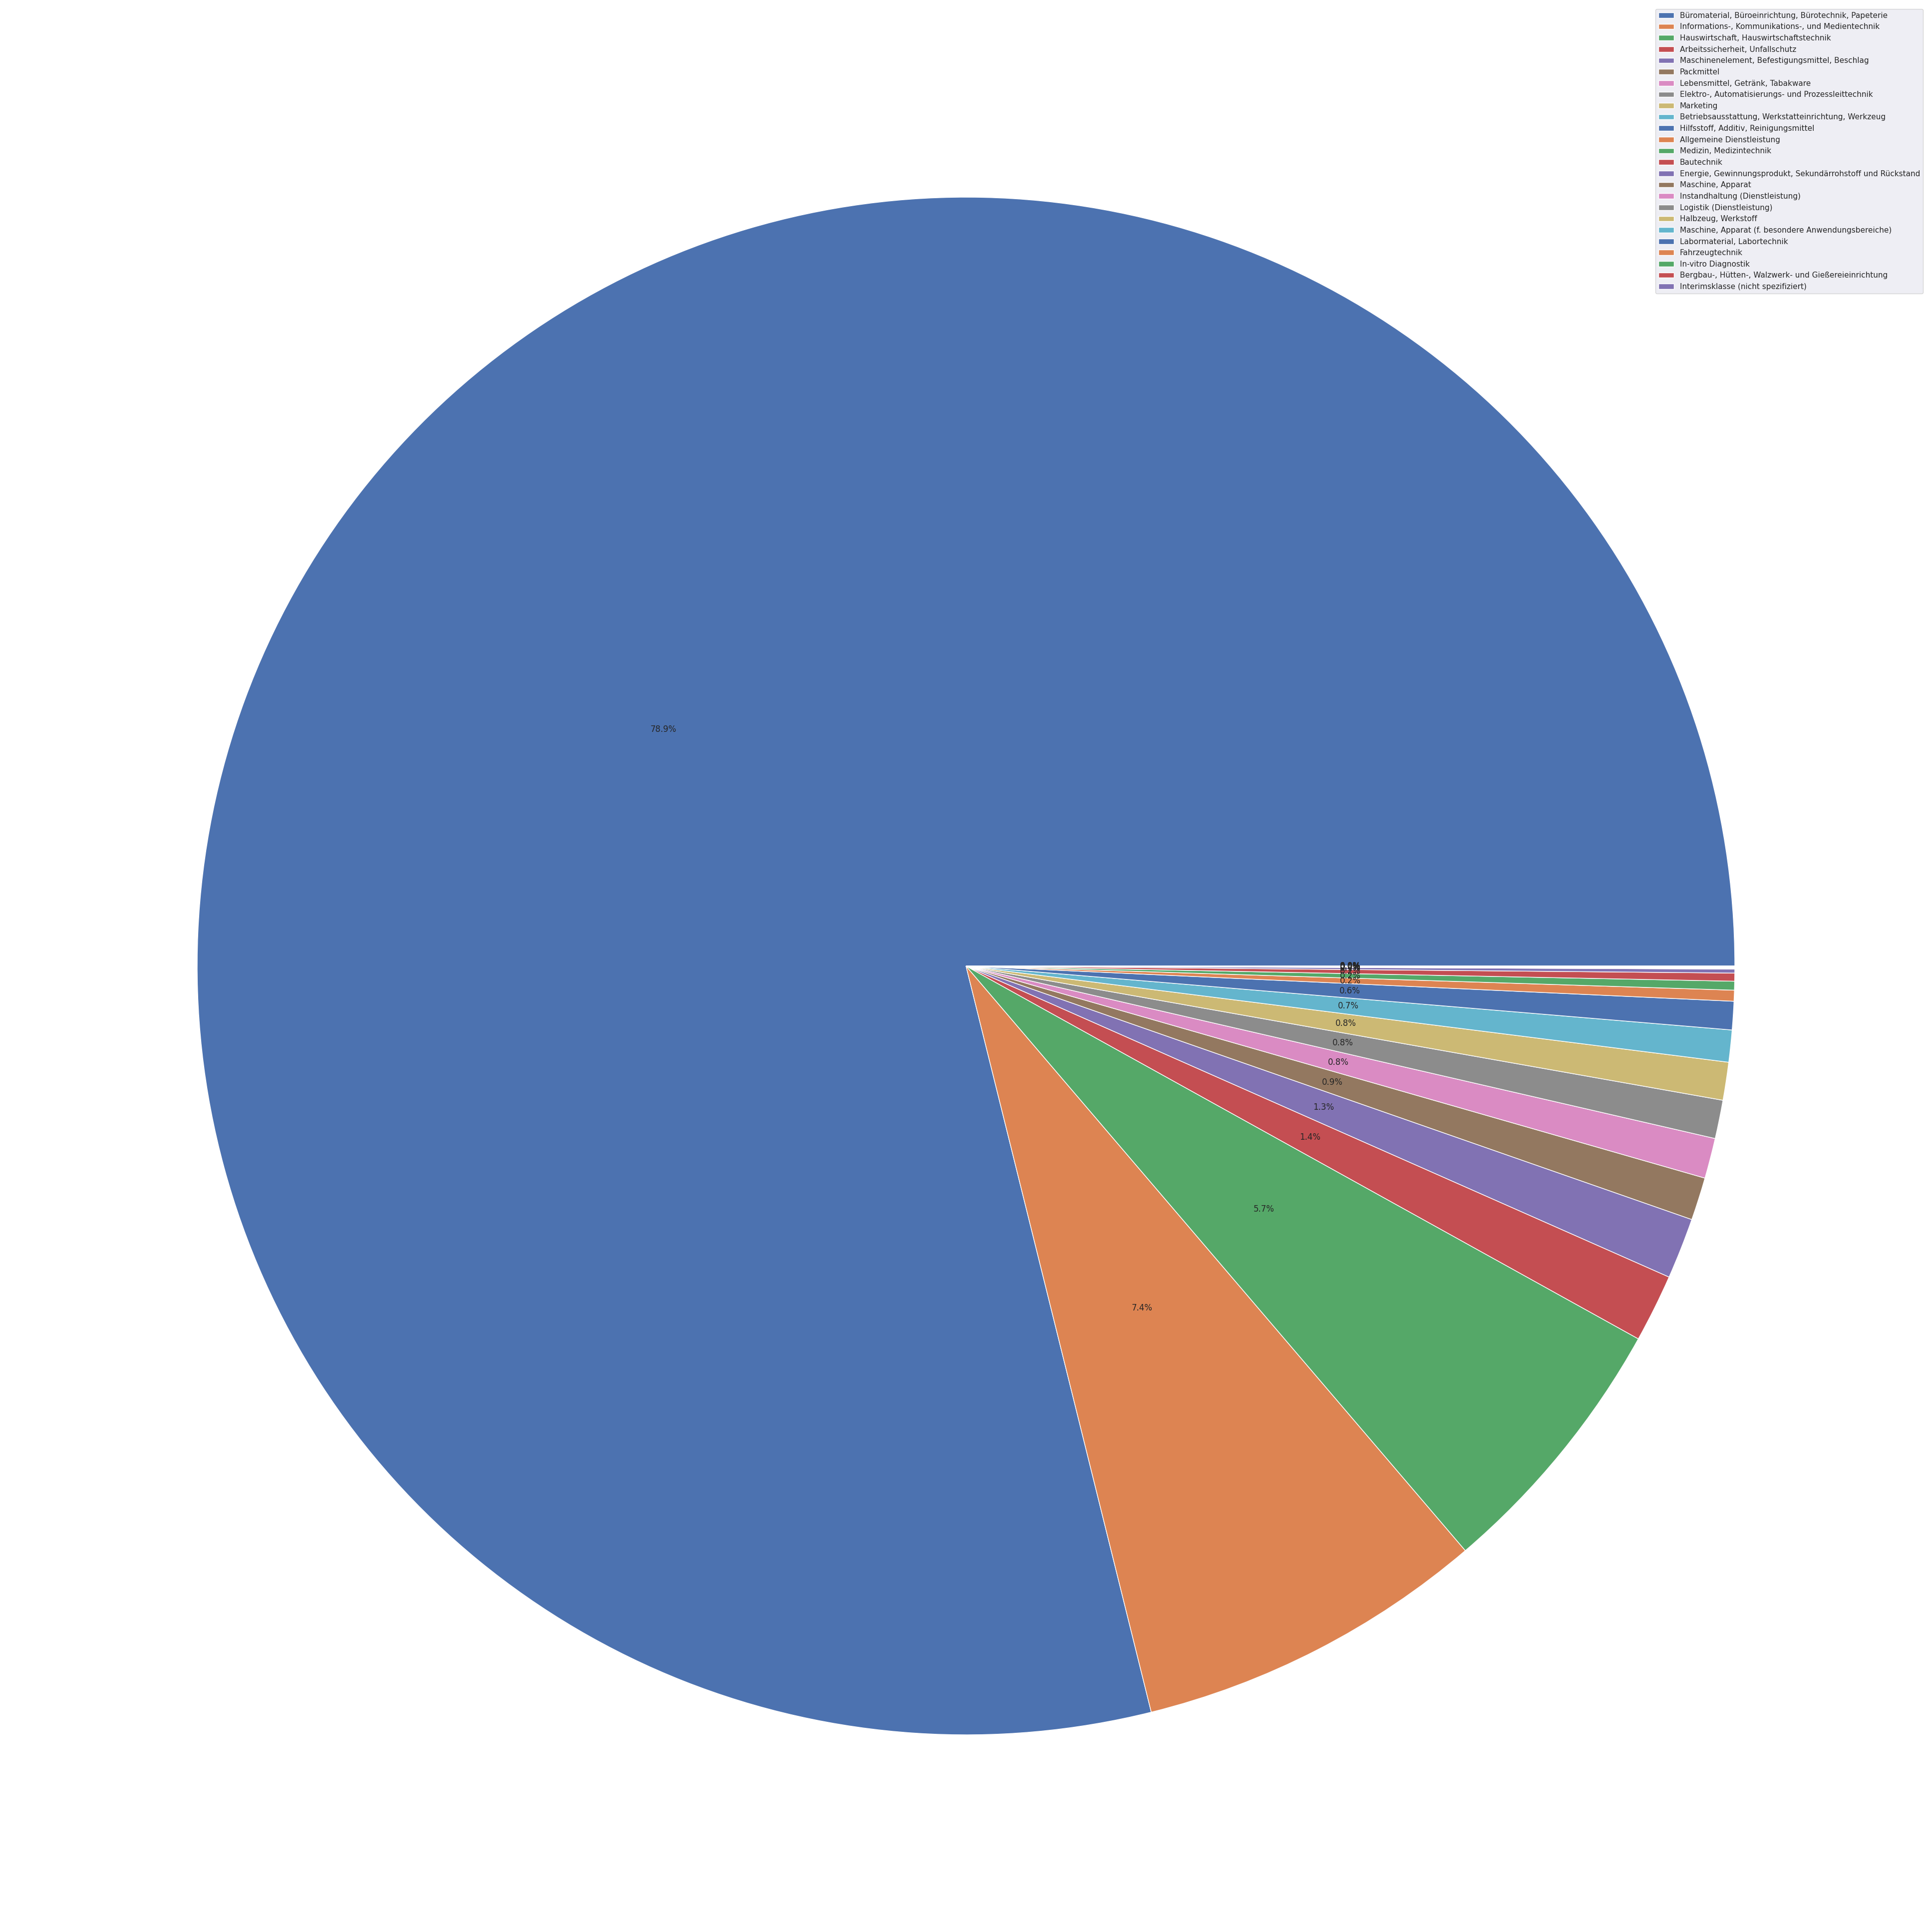
\includegraphics[width=1\linewidth]{level1_piechart}
	\caption{Percentage of products in each category in level 1}
	\label{fig:level1}
\end{figure}

\begin{figure}[H]
	\centering
	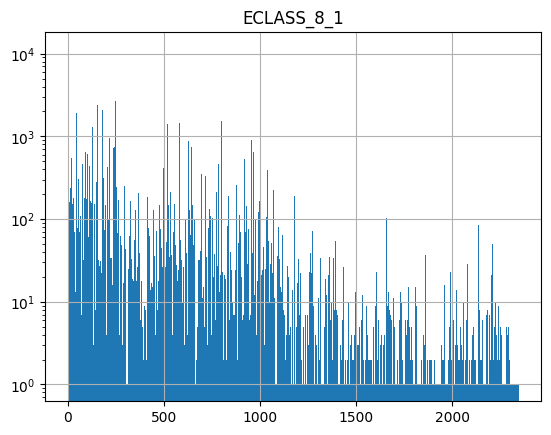
\includegraphics[width=1\linewidth]{level4}
	\caption{Logaritmic histogram of products in each category in level 4}
	\label{fig:level4}
\end{figure}

Despite these difficulties, addressing the dataset's complexity provided a deeper understanding of product descriptions and their inherent characteristics. 



\section{Pre-processing}

This section takes a look into the challenges and consequences of our pre-processing steps. We will dive into the process of finding examples for few-shot prompting and category descriptions, addressing how each decision impacts the subsequent phases of our experiment.


\subsection{Qualities and Challenges of Finding Product Descriptions for using as shots}

The decision to source product descriptions from Amazon provided both benefits and challenges in the search for diverse and extensive data. One distinguishing feature of Amazon product descriptions is their structure, which is frequently presented as bullet points highlighting key features. While this format aligns with the e-commerce platform's emphasis on clarity and conciseness, it presented challenges in generating coherent and flowing product descriptions. \cite{Team_2023}

The benefit of automation was invaluable in the data collection process. The vast array of Amazon products enabled automatic extraction of descriptions across a wide range of categories, resulting in a rich and diverse dataset for analysis. This automated approach simplified data collection, allowing for scalability and efficiency.

However, the structured nature of Amazon listings presented difficulties in terms of the desired format for product descriptions. Descriptions were frequently divided into bullet points or short statements, rather than a cohesive paragraph providing a narrative.  As a result, they had a negative impact on the coherence of the generated descriptions. When generating product descriptions, our model struggled to follow our intended format because of this mismatch.


Furthermore, despite Amazon's abundance of products, a few categories posed difficulties in finding appropriate examples. Obtaining diverse and representative samples became more challenging in cases where certain categories had limited representation or unique product categories. 


However, incorporating product descriptions from e-commerce websites that align with our research goals presents a promising avenue for enhancing the quality of our generated text. By manually searching German e-commerce platforms for product descriptions within the same category, we can curate a dataset that better suits our objectives. For instance, when focusing on a single product and exploring various e-commerce sites, we observed that employing a one-shot approach tends to yield more favorable results compared to a two-shot and zero-shot approach. The two-shot method often led the model to duplicate descriptions, lacking creativity and failing to tailor the content to the specific product.


\begin{center}
	\fbox{\begin{varwidth}{\textwidth}
			Die hohen Qualitätsstandards werden durch eine fachmännische Aufarbeitung des Tanks gewährleistet und garantieren somit ein optimales Druckergebnis bei gleichbleibender Qualität.Der neue Tintenspeicher wird nach den höchsten Standards aufbereitet,sodas er in seiner Funktion nicht eingeschränkt wurde! Das Ergebnis sind langlebige Drucke wie am ersten Tag zu günstigen Preisen.
			
	\end{varwidth}}\par
	\captionof{Example}{\label{exmaple-manual-description} An example product description generated for the sample product (\autoref{exmaple-product}) using the manually generated one-shot with category description. evaluation of this product description results in getting correctly classified by the PBS class classification model and a Flesch reading ease score of 20.38}
\end{center}

However, it's crucial to acknowledge the challenges associated with this manual approach. The process of manually sourcing descriptions from different websites is labor-intensive, time-consuming, and impractical for large datasets with numerous categories, as is often the case in e-commerce. We encountered these challenges firsthand when searching for product descriptions in the "toner" category, a more technical domain that theoretically provides richer descriptions. Despite our efforts, we found instances where product descriptions were represented by images or were entirely absent. As anticipated, this approach would pose greater challenges for a more general product category like "pen", where websites typically do not offer detailed product descriptions. This underscores the difficulty and limitations of manual data curation and emphasizes the potential benefits of automating the generation process for e-commerce websites, where our approach may offer a role in providing scalable and efficient solutions.

\begin{center}
	\fbox{\begin{varwidth}{\textwidth}
			Produktname: Brother Multipack TN243CMYK Toner 3,\\
			Produktkategorie: Toner, Tonereinheit (Laserdrucker, Kopierer),\\
			Katagoriebeschreibung: Pulver, das in Laserdruckern und Fotokopierern verwendet wird, um den gedruckten Text und die Bilder zu formen,\\
			Produktbeschreibung :Das Original Brother TN-243CMYK Value Pack beinhaltet jeweils eine Tonerkartusche in Schwarz, Cyan, Gelb und Magenta. Die Tonerkartuschen und die Brother Drucker wurden aufeinander so abgestimmt, dass beste Ergebnisse in brillanten Farben erzielt werden. Die Kartuschen sind leicht zu installieren. Profitieren Sie von langlebigen und hochwertigen Ausdrucken.Brother berücksichtigt die Auswirkungen auf die Umwelt in jeder Phase des Lebenszyklus Ihrer Tonerkartusche und reduziert den Abfall bei der Entsorgung. Unsere gesamte Hardware und alle unsere Tonerkartuschen sind so gebaut, dass sie die Umwelt so wenig wie möglich belasten.
	\end{varwidth}}\par
	\captionof{Example}{\label{exmaple-manual-shot} An example shot generated for the sample product (\autoref{exmaple-product}) from German e-commerce websites}
\end{center}



Although using shots from our dataset (Detailinformation feature) for evaluation seemed promising at first, we decided against it due to certain limitations. The shots lacked the structured format we desired and were mostly about the delivery process, making them unsuitable for our specific analysis. Furthermore, selecting the most representative or optimal description for evaluation becomes difficult in categories with a large number of instances. Given these constraints, Amazon was the best choice for our prompt shots. 



\subsection{Shots from unrelated vs related category}
In the investigation of the influence of shots from unrelated versus related categories on the prompt structure, our results consistently favored the use of related category shots. The class classification metric revealed that prompts incorporating shots from a related category, especially in the one-shot scenario, outperformed those with unrelated category shots. This trend was further confirmed in human evaluation, where the related category prompts showcased a more coherent and contextually appropriate generation compared to the unrelated category. The challenge with unrelated category shots lies in their potential to introduce confusing information, leading to descriptions that may not align with the intended product category. This emphasizes the significance of carefully selecting shots to guide the model effectively in generating accurate and contextually appropriate product descriptions.

\subsection{Category description: with or without}

The inclusion of category descriptions in our study played a significant role in influencing the performance of our models. Across various scenarios, we observed that configurations with category descriptions generally outperformed those without, as evidenced by both class classification accuracy and Flesch reading ease scores. Notably, the zero-shot approach with category description emerged as the optimal setup, showcasing its effectiveness in generating accurate and readable product descriptions.

The improved performance with category descriptions suggests that providing additional context about the product category aids the model in better understanding the intended context. This contextual information appears to enhance the coherence and relevance of the generated descriptions, resulting in more accurate classifications. The positive impact on Flesch reading ease scores further emphasizes that incorporating category information contributes to the overall readability and linguistic quality of the output. This finding underscores the importance of contextual cues in generating effective and informative product descriptions.

\section{Description generation}

This section looks into the complexities of description generation, covering the challenges and outcomes related to our hyperparameter and prompt engineering decisions. We discuss the difficulties faced when working with the German language and explain why we chose the Bloom model for our study.

\subsection{Bloom vs other LLMs}
Comparing GPT-2 and the Bloom model for German text generation reveals distinct differences in their performance. GPT-2, designed for English, struggles with linguistic accuracy in German, often introducing English phrases and lacking coherence. Even the version of GPT-2 trained on WECHSEL for German text falls short in performing well on our specific prompt. Despite its exposure to German data, GPT-2 struggles with linguistic nuances and fails to grasp the intricacies of the language when presented with our prompt. In contrast, the Bloom model, fine-tuned for German, produces more accurate and contextually relevant outputs.

The output from Mistral was non-existent, providing only new lines. Additionally, the fine-tuned version of Mistral on German language (em\_german\_mistral) generated a description with various product features. However, it included some inaccuracies, such as made-up model numbers.

In summary, for German product description generation, the Bloom model outperforms GPT-2 and Mistral, and therefore was selected as our primary model to conduct the studies employed in this thesis.

\subsection{Text generation in German vs English}

Our study into the relative performance of German and English text generation provides a few interesting results. We primarily focused on English text generation in our preliminary studies, leveraging the Bloom model with a total seen tokens of 366B. This huge model, distinguished by its size and complexity, demonstrated an extraordinary ability to generate coherent English descriptions while minimizing hallucinations. The extensive training data and model parameters were critical in achieving this level of competence.

Consider an English example where we tailored the prompt for a random Amazon product from the dataset \cite{amazon_data}. The generated description (\autoref{english-result}) highlights key features, is coherent and engaging with the customer.

{\tiny
	\begin{lstlisting}[breaklines=true, caption={prompt used for English text geneartion}, captionpos=b]
		
		Product Name:Electronic Snap Circuits Mini Kits Classpack, FM Radio, Motion Detector, Music Box (Set of 5) 
		Category:Toys & Games | Learning & Education | Science Kits & Toys 
		Product description:
		
	\end{lstlisting}
}

\begin{center}
	\fbox{\begin{varwidth}{\textwidth}
			\label{english-result}
			\begin{flushleft}
				This is the perfect way that you can make electrical work with kids. The best part about these products are they come packaged so easily! They’re easy-to-use because there’s no need any more complicated assembly or soldering skills needed.
				This product comes packed into two sets which include all five pieces required – including four small parts each - making it ideal as either individual projector set up/assembly toolkit / DIY electronics toy
			\end{flushleft}
	\end{varwidth}}\par
	\captionof{Example}{The product description generated in English using Bloom}
\end{center}

However, when we attempted to apply these findings to German text generation, we encountered significant difficulties. The Hugging Face platform's German version of the Bloom model is significantly smaller in scale. Unlike its English version, no larger or more complex than 7b model is currently available on this platform for German text generation. 

While the English Bloom model outperforms the German Bloom model, using this model and translating the results into German looked plausible. However, there are inherent risks connected with translation mistakes, which may jeopardize the quality and coherence of the resulting German product descriptions. We decided against this technique after thorough analysis in order to protect the integrity and reliability of our results.

The use of a more comprehensive and sophisticated model for English text generation aided in its improved performance. The availability of a large amount of training data, as well as the model's ability to capture subtle language nuances, were critical in producing high-quality text with fewer hallucinations. The limitations of the smaller German model, on the other hand, highlight the difficulties associated with adapting language models across different linguistic contexts. 

\subsection{Prompt style}

The incorporation of prompt style, particularly the addition of "formal," added a nuanced dimension to our investigation. While adhering to the optimal scenario of zero-shot with category description, the outcomes revealed an intriguing trend. The introduction of prompt style seems to have a negative effect, particularly on preventing hallucinations. Given the relatively small size of the model, it appears to be highly sensitive to alterations in the prompt. Another concern might be that the model may prioritize less important details over the product and category information. In the class classification metric, a noticeable decline in accuracy for levels 3 and 4 suggests that the formal style might disrupt the model's ability in capturing the essence of product and it's category (\autoref{fig:results_cc_prompt_style}). Additionally, the dip in the average Flesch reading ease score (\autoref{fig:results_flesch_prompt_style}) implies that the formal style could contribute to less accessible and less comprehensible outputs. These results underscore the need for cautious consideration when introducing prompt styles, as they can significantly impact the quality of generated product descriptions.

\subsection{Using different subsets of features}

Examining the influence of incorporating different subsets of features in the prompt, our study maintained consistency with the optimal setup of zero-shot with category description while adding brand and manufacturer information. Regarding class classification, the introduction of brand details exhibited a notable decrease in accuracy, particularly in deeper classifications (levels 3 and 4) (\autoref{fig:results_cc_feature}). The average Flesch reading ease score also experienced a slight decline (\autoref{fig:results_flesch_feature}), implying a potential trade-off between additional context and a possible reduction in precision and readability. Given the relatively small size of the model, it appears to be particularly sensitive to such complex features, potentially resulting in an increased risk of hallucinations. Additionally, the lack of dedicated tokens for manufacturer or brand information in the language model could explain the prompt's limited impact on generated product descriptions. The model may not effectively use such details, resulting in minimal influence on the text generation process. While the incorporation of more informative features might enhance the quality of product descriptions in certain cases, our findings suggest that, in the context of the PBS dataset, prioritizing the simplicity of category and product name may be more effective for generating accurate and clear outputs.


\subsection{Using different hyper-parameters for text generation}

In our exploration of hyperparameters' impact on the generated outputs, our primary focus centered on the temperature parameter, known for its pivotal role in balancing creativity, accuracy and quality in language model outputs. We compared three values—0.5, 0.8, and 1—while maintaining consistency in other aspects of the study, particularly the zero-shot approach with category description as the optimal setup. The outcomes indicated that a temperature of 0.8 produced the most favorable results in terms of class classification metrics (\autoref{fig:results_cc_temp}). Although the Flesch reading ease scores among the different temperatures showed close alignment, the average for 0.8 slightly outperformed the others (\autoref{fig:results_flesch_temp}). This underscores the significance of fine-tuning hyperparameters, particularly temperature, to achieve the optimal balance for generating accurate and readable product descriptions.


It was not possible to evaluate other hyperparameters, such as repetition penalty, because such an analysis is time-consuming. We chose specific values for these variables in our preliminary study and chose to preserve consistency across our studies. Furthermore, altering these parameters did not result in significant differences in the generated output, confirming our decision to focus on other vital elements.

\section{Post-processing}

In this section, we explore the phenomenon of hallucinations in the output of language models and try to figure out why they happen. Furthermore, we investigate the effects of our post-processing methods, offering insight into how these techniques reduce or alter the existence of hallucinations in the created content.

\subsection{Does rewriting actually help?}

In assessing the impact of the post-processing step on the generated outputs, a comparison between descriptions before and after post-processing was conducted, focusing on the optimal setup of zero-shot with category description. This study maintained consistency in all other parameters, revealing the effects on various metrics.


In considering the impact of the post-processing step on the generated outputs, it is evident that post-processing can have a positive influence on the overall readability of the text. However, the complex consequences of this step become apparent when examining its effects on other critical aspects, particularly class classification model's results.

The decrease in class classification accuracy suggests that post-processing may unintentionally remove critical details required for accurately categorizing the product class from the description (\autoref{fig:result_cc_postprocessing}). Because identifying and removing hallucinations is a difficult task, the post-processing step may mistakenly remove essential information about product features, compromising the classification of class of the product.

Furthermore, the removal of technical words during post-processing may contribute to a higher Flesch reading ease score (\autoref{fig:result_flesch_postprocessing}). However, it is critical to recognize that these technical terms are important when describing the complex features of a product related to technology. This highlights the difficulty in navigating the complex relationship between readability enhancement and essential information preservation during post-processing.

\subsection{Hallucinations}

The process of generating coherent and contextually accurate product descriptions using LLMs is limited by hallucination. In this context, hallucinations refer to the generation of text that contains fabricated or inaccurate information that differs from what is actually expected in a product description. Despite careful measures, the presence of hallucinations remains a difficult issue to address in the text generation pipeline.

Hallucination in LLMs is a complex problem with multiple contributing factors. One significant factor is the distribution shift between training and test data, which causes gaps that result in the generation of nonsensical or inaccurate content during inference. The lack of human supervision in guiding the model's responses, combined with a lack of alignment example coverage, increases the risk of hallucination. Flaws in the training mechanisms of LLMs can lead to the generation of content that deviates from its intended content. This hallucinatory output frequently displays a high level of confidence, making it difficult to distinguish between accurate and fabricated information. The two types of hallucinations are intrinsic and extrinsic. Intrinsic hallucinations contradict the original material, and extrinsic hallucinations lack verification. Moreover, as a consequence of inherent knowledge gaps in LLMs, nowadays LLMs are particularly prone to producing hallucinations, complicating the task of refining their outputs to align with factual and contextually accurate information. Despite ongoing research efforts, the precise causes of hallucinations remain unknown, emphasizing the complexities of mitigating this phenomenon in LLMs. \cite{Bilan_2023}  \cite{agrawal2023knowledge}

Furthermore, the size of the language model has a significant impact on vulnerability to hallucination. Smaller models, with fewer parameters and less extensive training, are more likely to produce hallucinatory outputs. Smaller models are more likely to generate content that deviates from the truth due to their limited ability to capture intricate patterns and subtle distinctions in data. \cite{Bilan_2023}  \cite{agrawal2023knowledge}

Overall, the problem of hallucination in generated text has a direct correlation with the complexity of language models, diversity of training data, and trade-offs between creative and accurate predictions. Although we have a two-step mitigation strategy, we must acknowledge the possibility of leftover hallucinations. For future work, there is potential to explore and develop more advanced methodologies that achieve an improved balance between maintaining an informative description and reducing the hallucination.

\section{Evaluation}

In this section, we turn our attention to the evaluation of our findings. We analyze the complexities of our chosen assessment criteria, analyzing their reliability and effectiveness in predicting the quality of the generated descriptions. In addition, we discuss the difficulties experienced throughout the evaluation process.

\subsection{How reliable are the readability metrics?}

While readability metrics provide valuable insights into the ease of reading a text, it's essential to acknowledge their inherent limitations. These metrics, including the Flesch Reading Ease score, offer a quantitative measure of text readability based on factors like word syllables, frequencies, and lengths. However, they are not infallible. One notable limitation is their sensitivity to technical terms, which are often integral to product descriptions. Technical language might impact readability metrics, even if the content is appropriately tailored for a specific audience.

Moreover, readability metrics focus on individual words and their characteristics, neglecting the broader context in which words are situated. They do not consider the interconnectedness of words, sentence structures, or the overall context of the text. Despite these constraints, readability metrics serve as a useful starting point for evaluating the accessibility of product descriptions, providing a quantitative benchmark for readability, although with an awareness of their limitations.

\subsection{Why do we use flesh reading ease instead of other readability metric?}
The selection of the Flesch Reading Ease score as our primary readability metric is supported by several considerations. This metric stands out for its simplicity and ease of interpretation, offering a numerical value on a scale of 0 to 100. Its widespread usage across various fields, coupled with its focus on general audiences, aligns with our goal of creating accessible product descriptions. Additionally, being language-independent ensures consistency in measurement across multilingual datasets. Flesch Reading Ease, tuned to assess clarity and simplicity, resonates well with our objective of crafting comprehensible product descriptions. While other metrics may offer detailed insights, the Flesch Reading Ease score's broad applicability and simplicity make it a fitting choice for evaluating readability in our context.

\subsection{How reliable is the class classification metric?}

Discussing the reliability of the class classification metric, our PBS model achieved a 67\% accuracy rate on descriptions within the sample dataset. This result indicates that the model does not consistently make accurate classifications and may struggle to infer the correct class from human-generated descriptions. While the model is not flawless, it serves as a valuable sanity check to ensure that product information is adequately conveyed in the descriptions. The metric becomes a useful tool for confirming that a person reading the description can reasonably infer the intended product category, adding a layer of confidence to the comprehensibility and relevance of the generated content. Despite its imperfections, the class classification metric provides a practical means of assessing the model's effectiveness in aligning descriptions with their respective product categories.




\subsection{Compound words in German and vectorization of them}

Navigating the intricacies of German compound words posed a considerable challenge in our process. Unlike English, where words are typically separated by spaces, German often strings words together to form compounds. We experimented with various approaches, including utilizing methods like "Simple Compound Splitting for German"\cite{Compound_Splitting_German} but encountered limitations in their effectiveness. Ultimately, due to the complexity and lack of reliable solutions, we opted for a two-step translation process. Initially translating German words to English allowed us to separate compounds into individual words. Subsequently, translating these individual words back to German provided a workable solution, even though it introduced a slight risk of translation errors. Notably, this method proved more effective, especially when dealing with technical terms where translation errors were minimal.

\subsection{Bloom based coherence metric}

The coherence metric, derived from the G-EVAL framework for NLG evaluation, introduces an innovative approach to assessing the coherence of generated text using LLMs \cite{liu2023geval}. We implemented the same concept but using the German bloom model(\autoref{german-bloom}). However, when applied to our study, several challenges and limitations came to light. Firstly, the metric relies on the same model that produced the descriptions to rate their coherence, introducing a potential source of bias. Additionally, we encountered instances where the model generated non-numeric characters, such as '*' or '(', instead of providing meaningful scores. This unpredictability raised concerns about the reliability of the metric.

Furthermore, upon closer examination of the results, a notable lack of variance in the model's scores became apparent. Despite human evaluations highlighting substantial differences in coherence among descriptions, the model consistently assigned similar scores. This uniformity raised questions about the metric's ability to capture differences in coherence, particularly when human evaluation indicated clear distinctions.

An additional complexity arose from the seemingly arbitrary nature of the model's scoring logic. In some cases, descriptions rated lower by the model were perceived as more coherent in human evaluation, creating inconsistencies in the assessment process. This lack of alignment between the model's scoring and human judgment further called into question the reliability and interpretability of the coherence metric.

Considering these challenges and uncertainties, we made the decision not to incorporate the coherence metric into our overall evaluation. While the metric offers a promising avenue for evaluating coherence in G-EVAL framework, our specific application revealed practical difficulties that hindered its effectiveness in providing meaningful and reliable assessments of the generated product descriptions.

\section{Time complexity}

The time complexity of our pipeline is an important factor to consider when assessing the efficiency of the product description generation process. The pipeline takes about two hour to complete the generation of descriptions for the set of 100 products in our study. This time span includes everything from pre-processing, generating the prompt, and processing the model's outputs to post-processing and evaluating the results.The current approach's inability to scale up is clear, as generating descriptions for one million products—a relatively small quantity for an e-commerce website—would take around 833.33 days. Addressing time constraints remains an important focus for potential improvements in the efficiency of our product description generation pipeline as we continue to explore optimizations and enhancements in our methodology.

\section{Future work}

There are various chances to improve and enhance the approaches used in this study when thinking about potential directions for future research. By addressing these factors, the created product descriptions may be more applicable and effective overall.

In our sampling approach, we randomly selected 100 products from our extensive dataset to conduct evaluations and analyses. While this method provides a diverse set of products for assessment, there could be potential improvements in the representativeness of the sampled data. An alternative strategy, which was considered but not implemented due to time constraints, involves clustering the dataset and selecting products located closer to the centroids of the clusters. This approach might offer a more balanced representation of the dataset, addressing potential biases introduced by random sampling. Exploring such clustering-based sampling methods could be a valuable avenue for future research, allowing for a better understanding of model performance across different categories and characteristics within the dataset.

Additionally, implementing an interface that allows users to input the category name and product details for automatic product description generation holds significant potential, particularly for online shops. This interface could serve as a practical tool for e-commerce platforms, streamlining the process of creating compelling and informative product descriptions. Users could input essential details such as the category and product name, leveraging our developed pipeline to generate engaging and tailored descriptions. Such an interface would not only enhance the efficiency of product listing but also contribute to a more consistent and professional presentation of products across diverse categories. This could potentially lead to improved customer engagement and satisfaction in the online shopping experience.

Furthermore, exploring the ratio of active to passive sentences as an additional evaluation metric could provide useful insights into the quality of generated product descriptions. Analyzing the distribution of active and passive sentences can provide an improved grasp of the text's readability, engagement, and information conveying effectiveness. A higher number of active sentences, for example, often indicates more direct and engaging communication, potentially improving the overall appeal of product descriptions to customers. An imbalance toward passive constructions, on the other hand, may indicate a less dynamic and persuasive narrative. We could gain a better understanding of the linguistic characteristics that contribute to effective product descriptions by incorporating this metric into the evaluation process, ultimately refining and optimizing language models for improved performance.

Currently, there is a lack of specific metric to quantify the extent of hallucination in generated texts. While metrics such as BLEU can evaluate similarity to reference texts, they rely on predefined references, making them less effective at detecting hallucinations. Creating a metric specifically designed to detect and quantify hallucinations in text could be a useful avenue for future research. Such a metric would provide a quantitative measure of the reliability of generated descriptions, allowing for a deeper evaluation of the model's performance, particularly in the absence of reference descriptions. Integrating such a metric into the evaluation framework could help us better understand the behavior of the language model and guide future improvements in hallucination mitigation.

Moreover, it might be useful in the future to fine-tune the Bloom model to generate German product descriptions specifically. Models that have been fine-tuned for a specific language or domain often perform better, as they capture the intricacies and nuances of the target context better. However, it's crucial to acknowledge that this task was beyond the scope of the current thesis due to time constraints and resource limitations. 
%\subsection{Comparison two different product and generating a text for it}

Finally, exploring the relative similarity against all categories in our dataset for the class classification metric using BERT could provide valuable insights and enhance the metric's utility. Currently, a challenge lies in the absence of a calibrated accuracy metric, making it difficult to assess the reliability and correctness of the model's performance. Conducting further research to establish a robust evaluation framework for the class classification metric would contribute to its effectiveness, ensuring a more accurate and trustworthy assessment of the inferred product categories from the generated descriptions.